\documentclass[border=1cm,10pt]{standalone}

% I only need the arrows for this one.
\usepackage{tikz}
\usetikzlibrary{arrows}
\usetikzlibrary{decorations.pathmorphing}
\usetikzlibrary{decorations.markings}
\usetikzlibrary{trees}

\begin{document}

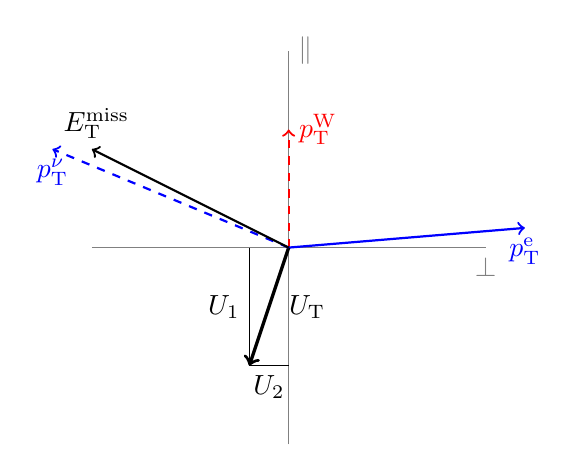
\begin{tikzpicture}[scale=.5] 
% Draw axes
\draw [gray] (-5,0) -- (5,0) node[below] {$\perp$};
\draw [gray] (0,-5) -- (0,5) node[right] {$\parallel$};

% Draw the boson
\draw[dashed,->,red,thick] (0,0) -- (0,3) node[right] {$p_{\mathrm{T}}^{\mathrm{W}}$};

% Draw the lepton
\draw[blue,->,thick] (0,0) -- (6,0.5) node[below] {$p_{\mathrm{T}}^{\mathrm{e}}$};

% Draw the Recoil
\draw[->,very thick] (0,0) -- (-1,-3) node[midway,right] {$~U_{\mathrm{T}}$};

% Draw the decomposed  Recoil
\draw[] (0,-3) -- (-1,-3) node[midway,below] {$U_{2}$};
\draw[] (-1,0) -- (-1,-3) node[midway,left] {$U_{1}$};

% Draw the Neutrino
\draw[dashed, blue,->,thick] (0,0) -- (-6,2.5) node[below] {$p_{\mathrm{T}}^{\nu}$};

% Draw the MET
\draw[->,thick] (0,0) -- (-5,2.5) node[above] {$~E_{\mathrm{T}}^{\mathrm{miss}}$};


\end{tikzpicture}

\end{document} 
